\begin{abstract}
A deployed model is replaced or adapted, and the team wants to know, as labels trickle in, whether its decisions cost more than a reference policy's.
Labels are expensive, so the monitor must choose which events to pay for.
We study this selective-label harm monitoring problem with anytime-valid betting e-processes and a pre-registered protocol.
Querying only the events where the two policies disagree raises evidence growth by $7.20\times$ at matched label spend
(95\% interval $6.88$--$7.55$) and wins $100$ of $100$ discordant detection comparisons at a $5\%$ budget.
A closed-form growth calculation that gives each arm its own support bound predicts the gain within $15\%$ at every budget.
When a policy intervention raises disagreement from $8\%$ to $41\%$, past-paced gating keeps the monitor running $1.9\times$ longer
than fixed-rate gating at identical label counts, detects equally often, and takes $1.4$--$2\times$ longer to alarm.
A sweep over $5$ intervention strengths and $4$ budgets maps where detection succeeds: at budgets of $5\%$ or less every selective monitor stays
below $0.30$ detection, while at $20\%$ they reach $0.87$ to $0.99$ once the intervention is moderate or stronger.
Null calibration passes on $2{,}000$ streams per cell, and on four real electricity-demand paths the monitors raise no false alarms and
detect injected under-procurement as fast as full feedback from a $5\%$ budget.
\end{abstract}

\section{Introduction}\label{sec:intro}

Models in production are retrained, patched and re-thresholded, and each change raises the same question: is the new
policy making decisions that cost more than the one it replaced? The answer lives in labels, and labels arrive late and at a price.
A fraud team pays an analyst per case, and a grid operator learns the cost of an under-procured reserve only after the day has passed.
A monitor for this problem must stay valid while the team watches continuously, and it must decide which events deserve a label.

Anytime-valid betting e-processes meet the first requirement. They bound the false-alarm probability at every stopping time and
are used to monitor risk and compare forecasters~\citep{waudbysmith2024,choe2022comparing,timans2025}.
The second requirement is a query rule. A deployed policy and its reference policy usually agree on most events, and on an agreement the paired cost difference is exactly zero.
Buying a label there carries no information. Paired auditing exploits this~\citep{mcnemar1947,discern}: spend labels only where the policies disagree.
That work establishes the label saving for certifying a single update at fixed confidence. What a monitor operator needs on top of it is the evidence-growth
and detection-delay consequence at the operator's actual budget, and the behaviour of the query rule when the policy change itself moves the disagreement rate.

\begin{figure}[t]
\centering
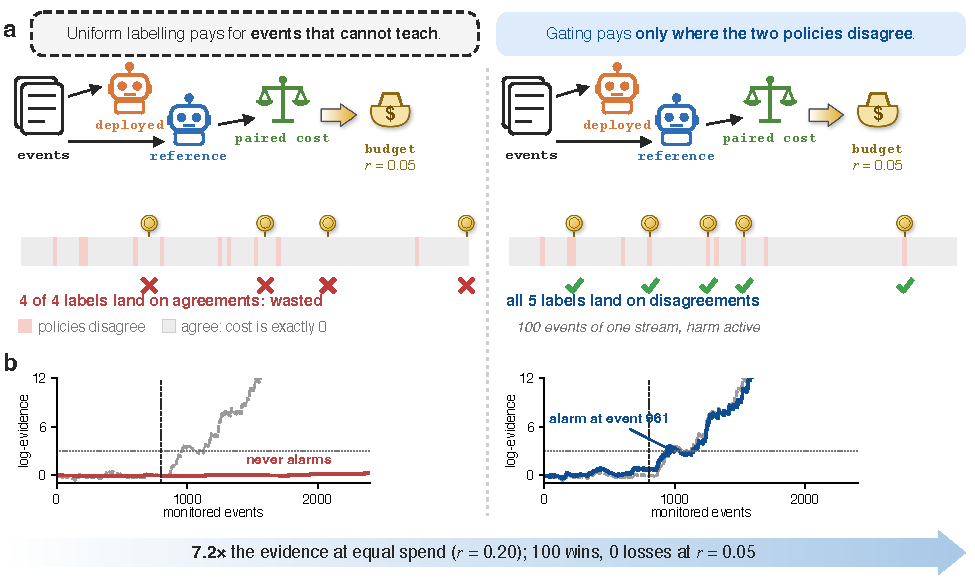
\includegraphics[width=\linewidth]{figures/fig_teaser.pdf}
\caption{Gating spends the label budget where labels can teach, and the evidence shows it. \textbf{a} A deployed and a reference policy score each event; where they agree the paired cost is exactly zero. Uniform labelling at budget $r=0.05$ puts all four of its labels in this window on agreements ($\times$), while gating puts all five on disagreements ($\checkmark$).
\textbf{b} Log-evidence on the same registered \texttt{boundary\_local\_harm} stream (seed $58400000$): gated labelling crosses the alarm threshold after harm onset (event $800$) at event $961$, matching full feedback, and uniform labelling never alarms. Panel a's robots and scales are schematic; the strips and curves are real.}
\label{fig:overview}
\end{figure}

We address both with a pre-registered study of selective-label harm monitoring. Our contributions are:
\begin{itemize}
\item At matched label spend, disagreement gating grows evidence $7.20\times$ faster than correctly bounded uniform labelling at a $20\%$ budget
(95\% interval $6.88$--$7.55$) and wins $100$ to $0$ in discordant detection comparisons at $5\%$ ($p=7.9\times10^{-31}$), with null calibration on $2{,}000$ streams per cell.
\item Per-event log-growth of an inverse-propensity betting e-process, computed with each arm's own support bound,
predicts the measured growth ratios within $15\%$ at all four budgets ($20.0/19.7/15.5/7.6$ against $17.5/20.6/14.7/7.2$).
The variance argument gives $\min(1/\rho,1/r)$ and the support-bound range penalty accounts for the rest.
\item Pacing the query rate to past disagreement keeps the monitor alive longer under a policy intervention but does not change how often it detects,
and it lengthens detection delay by a factor of $1.4$ to $2$ through the same range penalty.
\item Over $2{,}000$ streams spanning five intervention strengths and four budgets, detection rises with both,
and at budgets of $5\%$ or less selective monitors stay below $0.30$ where uniform labelling detects nothing.
\item Eight regimes carry predictions and falsification criteria, evaluated against Timans GRAPA, Xu active betting, prediction-powered e-values, empirical-Bernstein engines and SR/CUSUM under identical gating, bounds, budgets and query coins.
\item On four electricity-demand paths, all $68$ registered null cells raise no alarm, and under injected under-procurement fixed gating matches the full-feedback median delay in all ten harm cells from a $5\%$ budget upward, using $338$ to $701$ labels.
\end{itemize}

Section~\ref{sec:prediction} derives the growth prediction, Section~\ref{sec:protocol} describes the registered protocol, Section~\ref{sec:gating} reports the gating results,
Section~\ref{sec:pacing} studies pacing and the label reserve, and Section~\ref{sec:eia} reports the real-data results.

\section{Related work}\label{sec:related}

\paragraph{Paired auditing of model updates.}
\citet{discern} certify that an updated model does not regress, labelling only sampled disagreements with an anytime-valid confidence sequence.
They prove validity under any predictable routing rule and label-complexity bounds of order $\rho^2/\epsilon^2$, with matching lower bounds, which save a factor $1/\rho$ over pairing-blind auditing.
Their analysis is at a fixed verdict $(\epsilon,\delta)$ on i.i.d.\ streams. We use the same support identity and measure the resulting evidence growth and detection delay at a fixed budget,
including after a policy intervention moves the disagreement rate.

\paragraph{Anytime-valid active labelling.}
\citet{xu2024active} build inverse-propensity e-processes for risk control under any predictable labelling policy and derive the growth-optimal policy,
with a range condition that ties the betting fraction to the minimum query probability. We apply that range condition to the paired, zero-cost-on-agreement setting,
where it explains both the gating gain and the effect of pacing, and study behaviour under policy-induced change, which their i.i.d.\ analysis leaves open.
\citet{active2sample} give an active sequential two-sample test whose optimal query targets classifier-confident points and whose gain is stated through mutual information.

\paragraph{Active and prediction-powered inference.}
\citet{zrnic2024active} allocate a label budget by model uncertainty to narrow confidence intervals, and \citet{sfyraki2026} give non-asymptotic sequential bounds
for an active prediction-powered mean under a fixed distribution, with a budget cap on the query probability. These results concern estimation. We study sequential testing
of a paired harm null, where the query rule has a free subset (the agreements) and the distribution changes because of the policy under watch.

\paragraph{Monitoring and comparison by betting.}
\citet{timans2025} monitor a bounded conditional risk threshold under unknown shifts; their null coincides with our paired-cost null after an affine score map, and their GRAPA
engine is among our comparators. \citet{choe2022comparing} compare forecasters by anytime-valid score differentials, and \citet{podkopaev2022tracking} track a single model's risk.
These methods observe every outcome. We add selective labels and a hard budget.

